Окно настроек содержит элементы интерфейса, которые позволяют правильно настроить программу для
работы с устройством считывателя. Окно разделено на две части соответствующими вкладками: <<Файлы/Метки/События>> и
<<Подключенные устройства>>.

\subsection{Вкладка: Файлы/Метки/События}

Активировав вкладку
<<Файлы/Метки/События>>, пользователь получает возможность изменять настройки приложения. Верхние две строки вкладки
позволяют открыть или создать новые файлы журнала и настроек. 

\begin{center}
    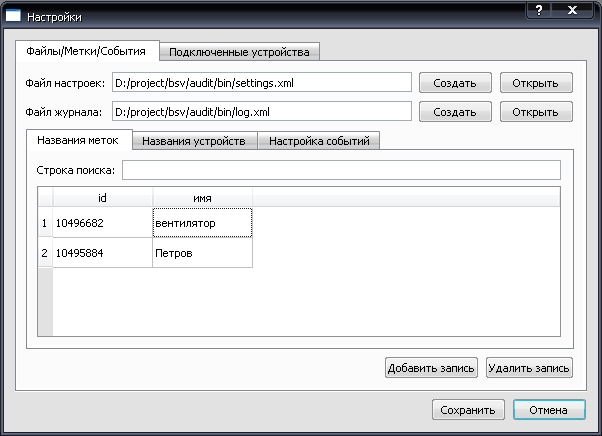
\includegraphics[scale=0.5]{img/settings_tag.png}
\end{center}

При открытии файла настроек, вся информация
из файла о настройках загружается в приложение и отображается в соответствующих местах интерфейса: информация о синонимах меток
ниже во вкладке <<Названия меток>>, информация о синонимах устройств во вкладке <<Название устройств>>, информация о 
настройках реакций на события во вкладке <<Настройка событий>>. Программа также загружает данные о 
настройках устройств, ранее сконфигурированных в программе.
Данные о настройках устройств используются в момент подключения новых считывателей. При подключении
нового устройства, программа проверяет, если у неё данные о его настройках, если да, то производится
автоматическое конфигурирование устройства. Таким образом, этап настройки необходимо производить только один раз
при наладке системы. В дальнейшем, требуется лишь загрузить соответствующий файл и система готова к использованию.

Для сохранения новых настроек приложения, необходимо нажать на кнопку <<Сохранить>> при активной вкладке
<<Файлы/Метки/События>>. При нажатии на кнопку <<Отмена>>, окно настроек закрывается.

При открытии файла журнала, информация о сохраненных в нем событиях отображается в окне монитора в виде таблицы.
Если файл хранит много данных, то показывается окно статуса процесса загрузки, где в процентах отображается
степень готовности операции чтения файла журнала.  

\subsubsection{Вкладка: Названия меток}

Для упрощения задач учета и контроля меток, в программе можно давать числовым идентификаторам меток
символьные имена. 

Вкладка <<Названия меток>> позволяет просматривать и редактировать информацию о синонимах меток. 
Редактирование осуществляется прямо в таблице, отображаемой во вкладке. Для удаления, необходимо выделить ненужную 
запись и нажать кнопку <<Удалить запись>>. Добавление новой записи производится посредством нажатия на
кнопку <<Добавить запись>>. Также в окне есть строка поиска, куда можно вводить ключевые слова, по которым
будет осуществлен поиск по таблице синонимов меток. Результаты поиска отобразятся сразу же в этой же таблице.

Чтобы сохранить изменения в файле настроек, нужно нажать кнопку <<Сохранить>>.

\subsubsection{Вкладка: Названия устройств}

Для упрощения взаимодействия с разными устройствами считывателей, в программе можно давать числовым идентификаторам устройств
символьные имена. 

Вкладка <<Названия устройств>> позволяет просматривать и редактировать информацию о синонимах устройств. 
Редактирование осуществляется прямо в таблице, отображаемой во вкладке. Для удаления, необходимо выделить ненужную 
запись и нажать кнопку <<Удалить запись>>. Добавление новой записи производится посредством нажатия на
кнопку <<Добавить запись>>. Также в окне есть строка поиска, куда можно вводить ключевые слова, по которым
будет осуществлен поиск по таблице синонимов устройств. Результаты поиска отобразятся сразу же в этой же таблице.

Чтобы сохранить изменения в файле настроек, нужно нажать кнопку <<Сохранить>>.

\begin{center}
    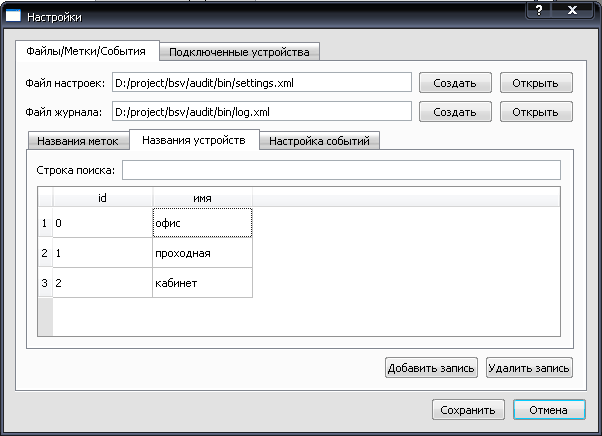
\includegraphics[scale=0.5]{img/settings_dev_name.png}
\end{center}

\subsubsection{Вкладка: Настройка событий}

Для выделения отдельных событий из всех случившихся, в программе можно настраивать определенную реакцию
на предполагаемое событие. 

Предусмотрено два вида событий: обнаружен новый таг либо таг потерян. На эти события возможно отреагировать двумя способами.
Либо выделить цветом событие в окне монитора, либо выдать сообщение о происшествии данного события.
В случае показа сообщения, программа регистрирует в файле журнала факт реакции оператора на него. Фиксируется закрытие
оператором окна с оповещением о событии.

Настройка реакций на события происходит путем редактирования таблицы в данной вкладке. Ячейки с номером канала, событием и реакцией
изменяются посредством выпадающих списков. Причем при выборе реакции <<выделить цветом>>, открывается диалоговое окно с цветовой палитрой, где
пользователь может выбрать необходимый цвет подсветки события. Остальные ячейки изменяются как текстовые поля. 

Для удаления, необходимо выделить ненужную 
запись и нажать кнопку <<Удалить запись>>. Добавление новой записи производится посредством нажатия на
кнопку <<Добавить запись>>. 
Чтобы сохранить изменения в файле настроек, нужно нажать кнопку <<Сохранить>>.

\begin{center}
    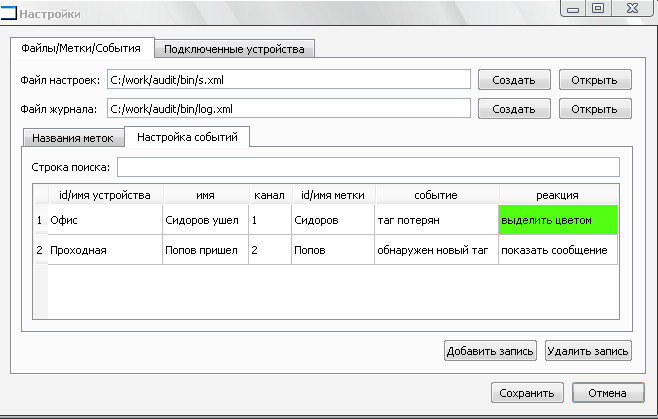
\includegraphics[scale=0.5]{img/settings_event.png}
\end{center}

\subsection{Вкладка: Подключенные устройства}

Элементы интерфейса на данной вкладке позволяют настраивать подключенные к компьютеру считыватели.
При нажатии на кнопку <<Найти устройства>>, программа отображает информацию о подключенных устройствах в
виде списка в верхней части окна. Если файл настроек содержит информацию по конфигурированию подключенных устройств, то
производится их автоматическая настройка. Активные устройства выделяются цветом в списке.

При нажатии на кнопку <<Синхронизировать часы>>, обновляется время внутренних часов для всех обнаруженных считывателей.
Чтобы поправить настройки для отдельного устройства, необходимо выбрать его щелчком левой клавиши мышки в списке.
После этого информация о текущих его настройках отобразится в нижней части окна. 

Можно сделать устройство активным, нажав на
<<Подключить устройство>>. Если данная кнопка находится в нажатом состоянии, то устройство уже активировано.
После активации, программа начнет считывать данные из его журнала транзакций и 
отображать их в окне монитора. Подключение и отключение каналов происходят по нажатию на кнопках <<Канал 1>>, <<Канал 2>>.
Если канал включен, то соответствующая кнопка отображается в нажатом состоянии.

Настройка считывателя в соответствии с заданными параметрами производится после нажатия на кнопку <<Сохранить>>.
Если есть необходимость внести эти настройки в файл настроек, то нужно переключиться на вкладку <<Файлы/Метки/События>>
 и нажать на кнопку <<Сохранить>>.

\begin{center}
    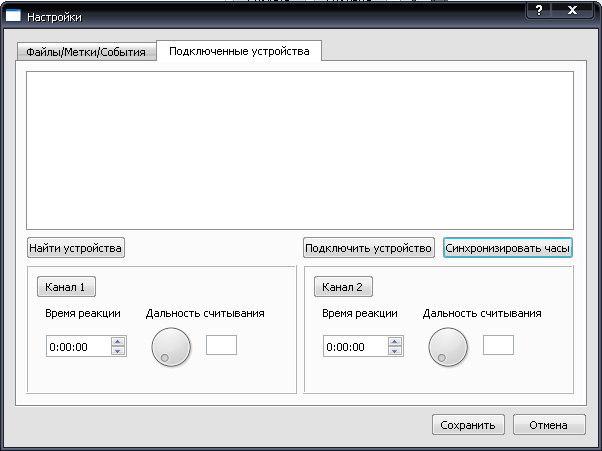
\includegraphics[scale=0.5]{img/settings_dev.png}
\end{center}
